\documentclass[sigconf]{acmart}

\settopmatter{printacmref=false} % Removes citation information below abstract
\renewcommand\footnotetextcopyrightpermission[1]{} % removes footnote with conference information in first column
\pagestyle{plain} % removes running headers

\usepackage{booktabs} % For formal tables


% Copyright
%\setcopyright{none}
%\setcopyright{acmcopyright}
%\setcopyright{acmlicensed}
\setcopyright{rightsretained}
%\setcopyright{usgov}
%\setcopyright{usgovmixed}
%\setcopyright{cagov}
%\setcopyright{cagovmixed}
\usepackage{graphicx}

\copyrightyear{2017}


\acmArticle{4}
\acmPrice{15.00}


\begin{document}
\title{TrailBlazer - Progress Report}
\subtitle{CSE6242 FALL2017}


\author{\textbf{Alexandre Palo}}
\affiliation{%
  \institution{Georgia Institute Of Technology}
  \streetaddress{North Avenue}
  \city{Atlanta} 
  \state{Georgia} 
  \postcode{30332}
}
\affiliation{%
  \institution{\'{E}cole nationale sup\'{e}rieure d'arts et m\'{e}tiers}
  \streetaddress{151 Boulevard de l'Hôpital}
  \city{Paris} 
  \state{France} 
  \postcode{75013}
}
\email{alexandre.palo@gatech.edu}

\author{\textbf{Guillaume Broggi}}
\affiliation{%
  \institution{Georgia Institute Of Technology}
  \streetaddress{North Avenue}
  \city{Atlanta} 
  \state{Georgia} 
  \postcode{30332}
}
\affiliation{%
  \institution{\'{E}cole nationale sup\'{e}rieure d'arts et m\'{e}tiers}
  \streetaddress{151 Boulevard de l'Hôpital}
  \city{Paris} 
  \state{France} 
  \postcode{75013}
}
\email{guillaume.broggi@gatech.edu}

\author{\textbf{Alex Mueller}}
\affiliation{%
  \institution{Georgia Institute Of Technology}
  \streetaddress{North Avenue}
  \city{Atlanta} 
  \state{Georgia} 
  \postcode{30332}
}
\email{alex.mueller@gatech.edu}

\author{\textbf{Tianyi Zheng}}
\affiliation{%
  \institution{Georgia Institute Of Technology}
  \streetaddress{North Avenue}
  \city{Atlanta} 
  \state{Georgia} 
  \postcode{30332}
}
\email{tianyi.zheng@gatech.edu}

\maketitle

\section{Introduction}

Right now there is no convenient web application to help bikers and hikers find enjoyable trails. The best option is something like Google Maps, but it is designed to go from a point A to a point B and it lacks crucial meta-information like trail conditions and difficulty. In order to find this information, users have to refer to additional websites which further complicates the process. Additionally, Google Maps does not have points of interest (POI) that are geared towards hikers. \textbf{(Heilmeier Q1, Q2)} Our goal is to create an application that not only helps bikers and hikers find trails but to also introduce them to unique and interesting POI that would not have seen otherwise.

\section{Related work}
Because there are no all-in-one applications that do exactly what we plan to do, there is little previous literature regarding similar applications. However, there is plenty of literature surrounding our project's component parts: data, database, backend, and user-interface.

All of our data is open-source or crowd-sourced. This leads to our major risks: users getting lost or injured. \textbf{(Heilmeier Q6)} Our map data is pulled from OpenStreetMap, which according to Haklay, has fairly impressive coverage. However, it is somewhat lacking in low-population areas (Haklay 2010). This could cause issues with finding accurate trail data. Our trail quality/difficulty and POI information are pulled from crowdsourcing sites that may have issues in information quality. One possible solution is to look at user reviews to determine data quality so that we can filter out low quality data (Allahbakhsh 2013).

As for the database, Amirian, et al. compared the performance and scalability of SQL databases, spatial databases (SQL with support for spatial data), and an XML document NoSQL database. NoSQL showed better performance in single and multiple geospatial feature retrieval queries (Amirian, et al. 2014). Agarwal, et al. also ran geospatial querying tests specifically comparing MongoDB and PostgreSQL (with PostGIS) databases. They found MongoDB performed on average 10 times better than PostgreSQL with PostGIS (Agarwal 2017). Additionally, MongoDB 's document structure makes it perfect for GeoJSON.

We considered two backend APIs: REST API and GraphQL API. In a REST API, the frontend is independent from the stateless backend. The backend also has a uniform data interface which is implemented such that it will respond to any request with minimal information from the client. (Fielding 2000) GraphQL is fundamentally different from REST. GraphQL is essentially a query language that allows a client to send requests to the server. Unlike REST, GraphQL requires that the client directly specifies what it wants from the server. This could make the communication between the client and the server more complicated but could also allow for more specific requests that could save computational resources. (Paris 2017)

The most promising algorithms for path generation were from Tarjan and Johnson. Tarjan outlined an algorithm that uses Dijkstra's algorithm to find the shortest path between nodes and uses depth-first search to find cycles/blocks that can be used as paths (Dijkstra 1959, Tarjan 1972). Johnson also designed an algorithm that finds all simple cycles in a directed graph (Johnson 1975).

In order to develop an effective UI, Rosenzweig says that we need to know the demographics of our users as well as how they will use our application. By investigating the use cases for our application, we can ensure that the the UX is as smooth as possible to our users (Rosenzweig 2015).

An expected benefit function built from a confusion matrix (Provost and Fawcett  2013, chap. 7) serves as a promising method to assess both our progress and the performance of our algorithm\textbf{(Heilmeier Q5)}. This function is a probabilistic tool that will allow us to guess how much value an algorithm adds when applied to a given population. It also allows us to compare different version of our algorithm against each other as well as against baselines. One level decision trees are often more efficient that more complex models, so it will act as a solid baseline for our model (Holte 1993). Google Maps results will also provide a good baseline.  If this method turns out to be too imprecise, we can use a Receiver Operating Characteristic graph that plots the true positive rate against the false positive rate (Provost and Fawcett, 2013 chap. 8).\textbf{(Heilmeier Q9)}

\section{Proposed method}
Users will select their start point and optional end point on a map in an online interface. These points will be passed to a backend REST API that was implemented using Python and Django. The API will then query the database for POI nearby the start and end points as well as for trails near those POI. These nodes (POI) and edges (trails) are then used to construct a graph using the networkx library. Tarjan's algorithm is then used to construct possible cycles with these nodes (POI) and edges (trails). We are using a MongoDB database hosted by MongoDB's Atlas program to hold this information. The API will then send the cycles and POI back to the online interface. The UI will then plot the POI as points on the map and display the cycles as trails the user can use to visit those POI. The front-end application, based on the React and Redux libraries, will be totally interactive in order to let the user see, assess, select, or modify solutions given by the algorithm.

One could argue that this could all be done by Google Maps. However, we are introducing three main innovations. First, our application will provide users with information and metadata about the trails that Google Maps cannot provide. For example, we will allow users to see the trail difficulty, the elevation changes, and other information that users would regularly have to visit other websites for. This information will be displayed on an adjacent D3 graph (see appendix: figure 1). Second, our POI will be focused purely on bikers and hikers. Instead of listing restaurants and gas stations like Google Maps, we will list geocaches and natural landmarks. Third, as mentioned before, we will be generating our paths using Tarjan's algorithm. \textbf{(Heilmeier Q3, Q4)}

The mapping data (trails, roads, etc.) was pulled from OpenStreetMap. Points of interest  and trails were scrapped from two websites, Geocaching.com and UtagawaVTT.com, respectively. These websites are crowdsourced and lists cache positions and descriptions or trail conditions and difficulties. We are currently looking for ways to check the quality of this data. Since caches and trails are manually uploaded from user's GPS systems, we can assume that they exist. Unfortunately, we do not always have user reviews to assess the data quality; however, the user interface will allow users to upload new data and give feedback. This will allow users to correct information and ensure that it is up-to-date.

The costs of this application are minimal. All of our data is free, and we will be hosting the backend on our own machines. The only cost will be for hosting the MongoDB database on MongoDB Atlas, which will cost \$10-\$20/month depending on how much data we collect. There is only about two months left in this course, so we expect to spend \$20-\$40 total for this project. \textbf{(Heilmeier Q7)}

\section{Experiments and evaluation}
Our project is currently in its alpha stage and is not at a point where where we can truly evaluate its performance. However, we are currently testing our application on a trial dataset. This trial dataset includes the trails and POI from a small area of France. Our current goal is to refine our application using this dataset while we accumulate more data. We are able to query the database and to display simple trails in the user interface (see figure 1).

\begin{figure*}
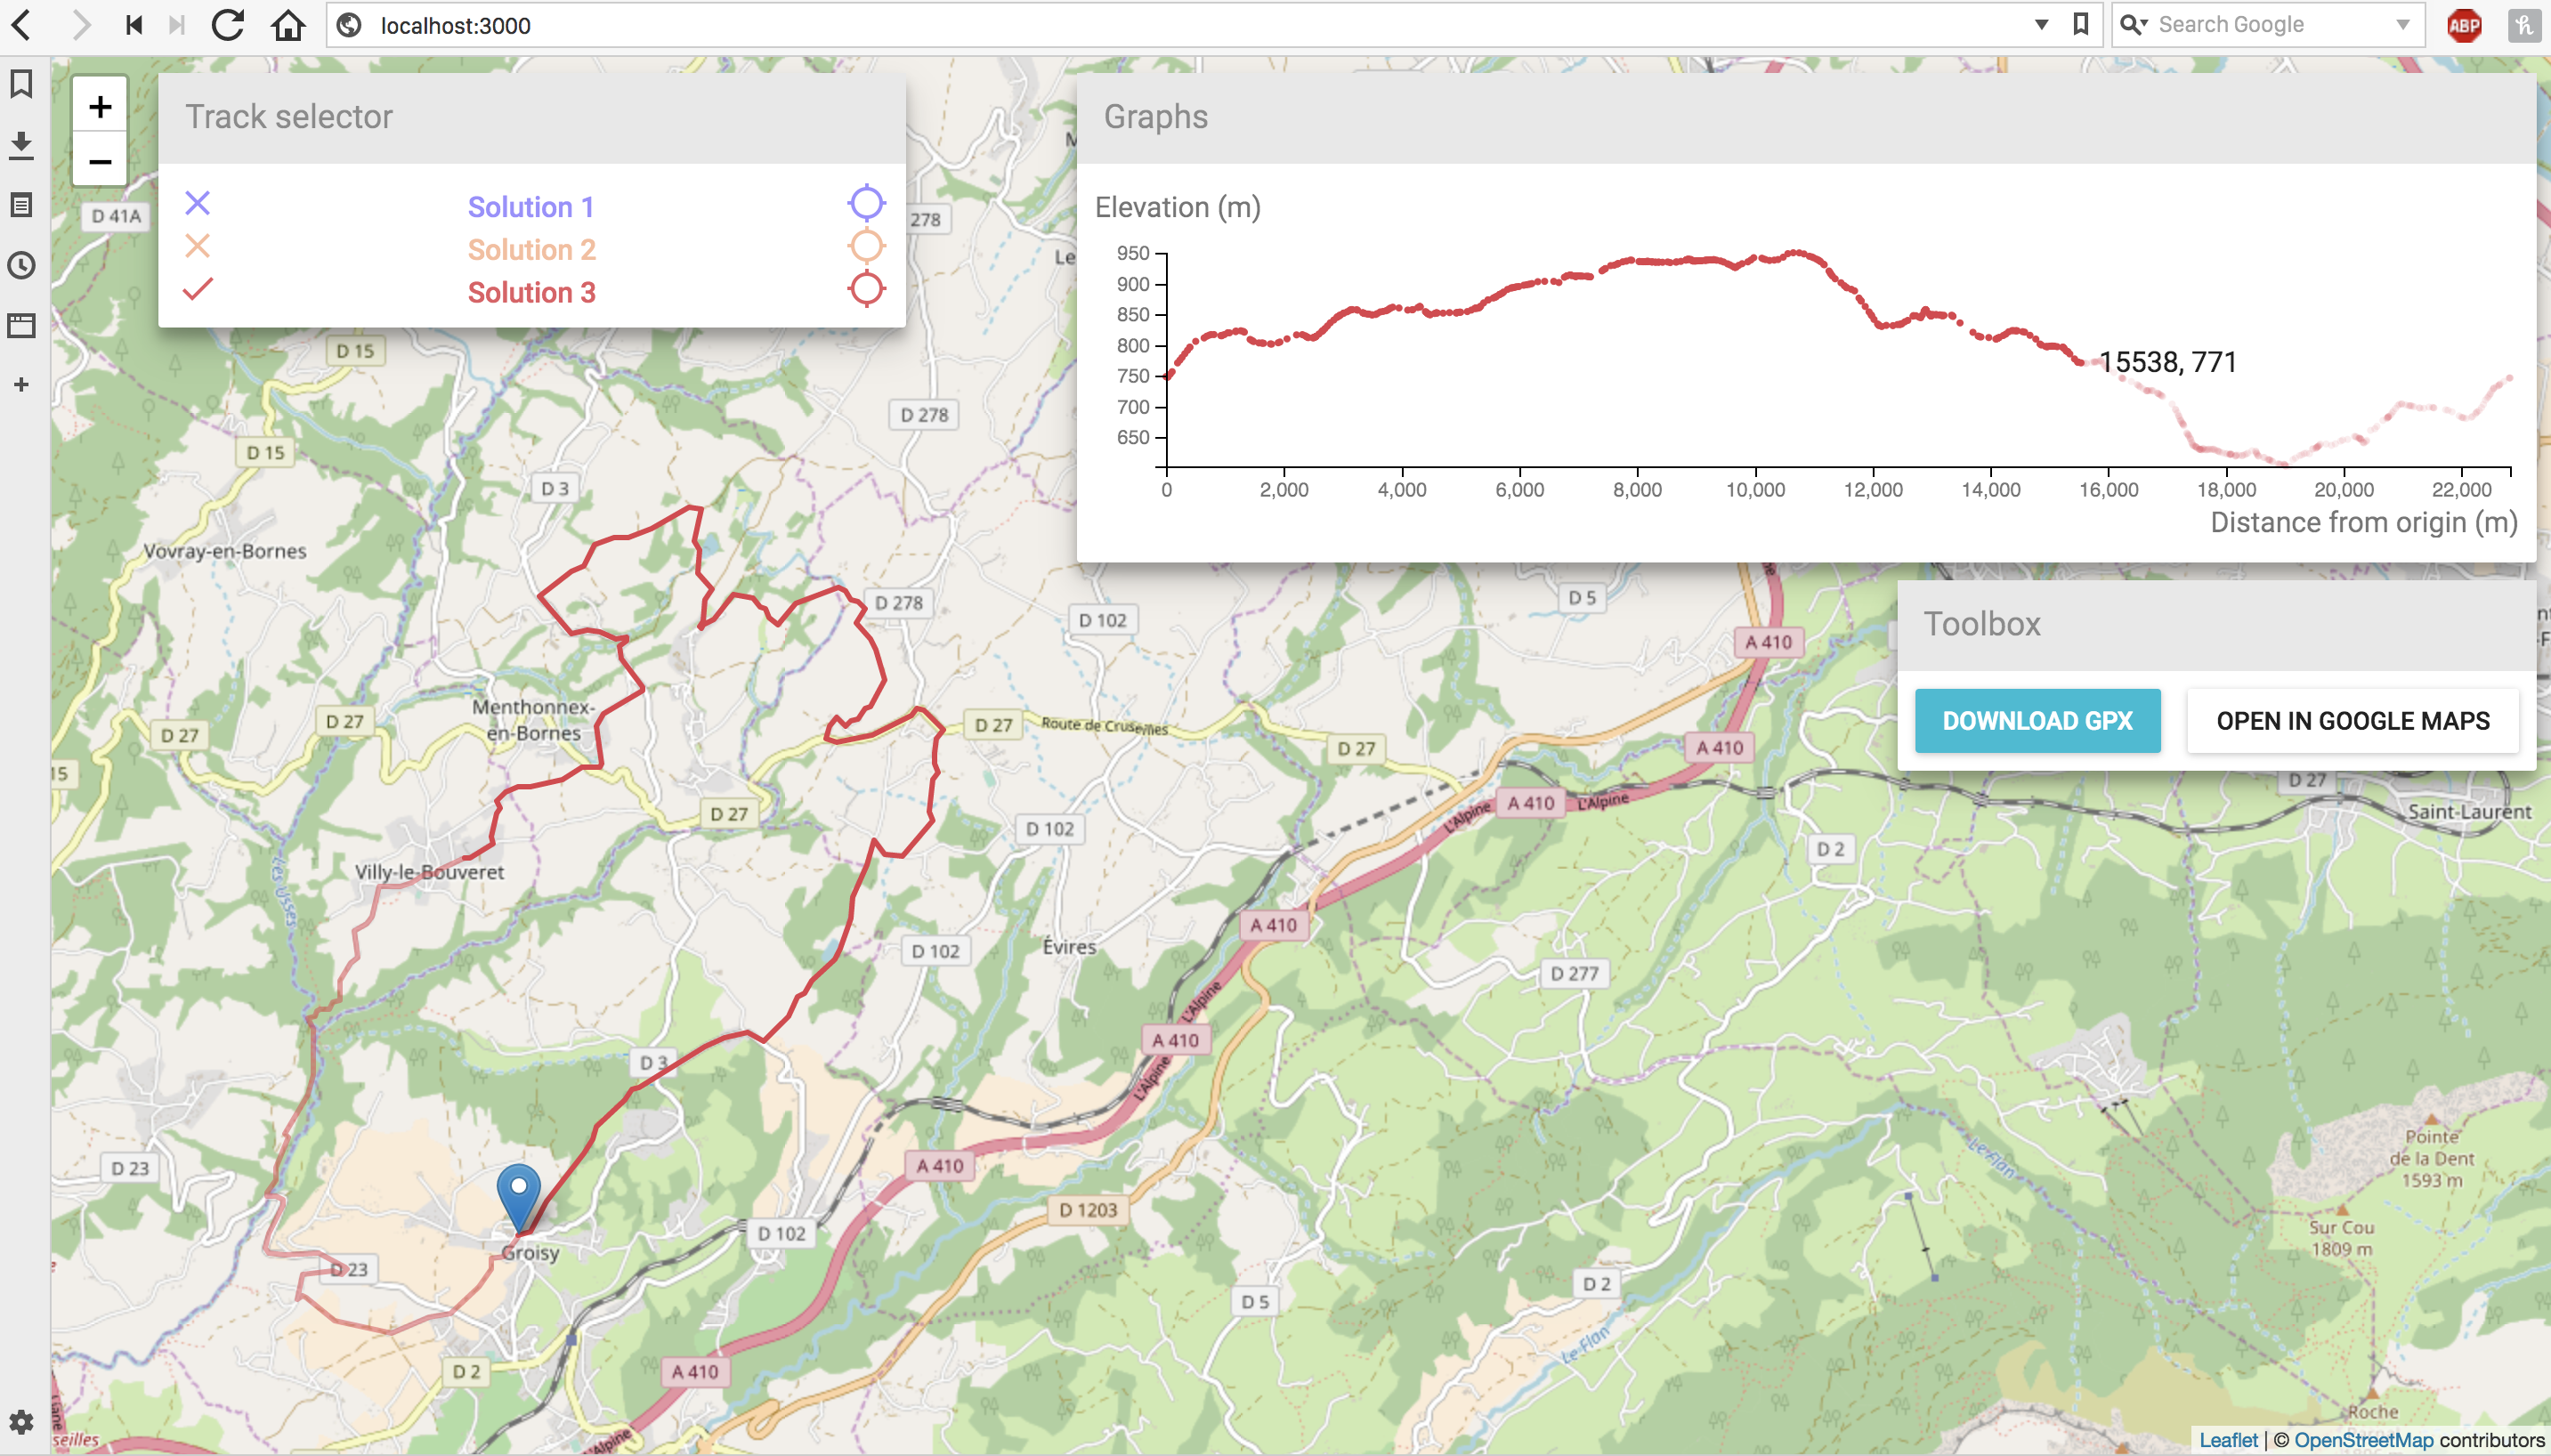
\includegraphics[scale=0.3]{current_frontend.png}
\caption{Current frontend design.}
\end{figure*}

There was no data API for either Utagawa VTT and Geocaching, so data scraping involved some reverse engineering because data access is reserved to members of those sites (see figure 2 for an activity flow). The database from UtagawaVTT represents more than 11,000 trails, mostly in France. It is 690 MB of data, mostly consisting of GPS coordinates.

\begin{figure*}
\includegraphics[scale=0.5]{scrapping_flow.png}
\caption{Scrapping flow.}
\end{figure*}

After the alpha stage,  performance will be evaluated using the expected benefit function and simple usability surveys. In these usability surveys we will give users a simple task to complete with our application, say, finding a good path between a start and end point that we provide to them. We will provide them with minimal instructions in order to determine whether or not our user interface is intuitive. Additionally, we will ask them to compare our application to other mapping applications that they use (Google Maps, Apple Maps, etc.). \textbf{(Heilmeier Q5)}

\section{Conclusion}

Admittedly, we are a little behind our target timeline. The component parts are all working independently, and now we are just smoothing out the information flow between them. There is an updated timeline based on our current progress in appendix A.

We are confident that we will be able to adhere to this new timeline now that we have a better idea of how long certain processes and elements of the project will take. \textbf{(Heilmeier Q8)} We have included additional information in the appendix, such as our previous timeline and activities of each group member as well as some figures.

\appendix
\section{Timelines}
\subsection{Current timeline}

\begin{itemize}
	\item November 13: Database, backend, and frontend connected and communicating
	\item November 20: Application functioning on small dataset
	\item November 24: Poster design complete
	\item November 27: Application polished and presentable for poster presentations
	\item November 30: Poster presentation, full dataset uploaded
	\item December 4: Final report complete
\end{itemize}

\subsection{Previous timeline}
\begin{itemize}
	\item October 23: Able to query locations from front-end, all data added to database
	\item November 6: Simple path generated and displayed based on user-provided start and end points
	\item November 10: Progress report due
	\item November 20: User can select options to impact path generation, continue to refine algorithm and front-end
	\item November 28: Poster presentation
	\item December 5: Project complete, final report due
\end{itemize}

\section{Work distribution}

\begin{itemize}
	\item Scraping and collecting data: Uttagawavtt, Geocaching (Guillaume)
	\item Cleaning and standardizing data (Guillaume, Alex)
	\item Designing our algorithm (Tianyi, Alexandre)
	\item Implementing the backend (Tianyi, Alex)
	\item Creating the front-end (Alexandre)
\end{itemize}

All team members have contributed similar amount of effort.

\section{Innovations}
\begin{itemize}
	\item Incorporating trail quality data
	\item Using Tarjan's algorithm to generate paths
	\item Scraping and providing points of interest specifically geared towards bikers and hikers
\end{itemize}

Further possible innovations we would like to implement if we have time:
\begin{itemize}
	\item Hikers can update trails and give feedback
	\item One can edit the trail he wants to follow directly in the interface (by drag and drop for example)
	\item One can export the trail to a gps thanks to a gpx file
\end{itemize}


\begin{thebibliography}{9}
\bibitem{} 
Agarwal, Sathak and KS Rajan. 
\textit{Analyzing the performance of NoSQL vs. SQL databases for Spatial and Aggregate queries.}. 
Free and Open Source Software for Geospatial Conference Proceedings 17, 2017.
 
\bibitem{} 
Allahbakhsh, Mohammad, Boualem Benatallah, and Aleksandar Ignjatovic.
\textit{Quality Control in Crowdsourcing Systems.}.
Web-Scale Workflow, 76-81, 2013.

\bibitem{} 
Amirian, Pouria, Anahid Basiri, and Adam Winstanley.
\textit{Evaluation of data management systems for geospatial big data}.
International Conference on Computational Science and Its Applications. Springer, Cham, 2014.

\bibitem{} 
Dijkstra, Edsger W.
\textit{A note on two problems in connexion with graphs}.
Numerische mathematik 1.1 (1959): 269-271.

\bibitem{} 
Fielding, Roy Thomas.
\textit{Architectural Styles and the Design of Network-based Software Architectures}.
Doctoral Dissertation, University of California, Irvine, 2000.

\bibitem{} 
Johnson, Donald B.
\textit{Finding all the elementary circuits of a directed graph}.
SIAM Journal on Computing 4.1 (1975): 77-84.

\bibitem{} 
Haklay, Mordechai.
\textit{How good is volunteered geographical information? A comparative study of OpenStreetMap and Ordnance Survey datasets}.
Environment and Planning B: Planning and Design 37 (2010): 682-703.

\bibitem{} 
Holte, Robert C.
\textit{Very Simple Classification Rules Perform Well on Most Commonly Used Datasets}.
Computer Science Department, University of Ottawa, 1993.

\bibitem{} 
Provost, Foster, and Tom Fawcett.
\textit{Chapter 7: Decision Analytic Thinking I: What Is a Good Model?}
Data Science for Business: What You Need to Know about Data Mining and Data-Analytic Thinking, O'Reilly (2013).

\bibitem{} 
Samer Buna.
\textit{All the fundamental React.js concepts}
Medium (blog), Aug 2017.
\\\texttt{goo.gl/LUMxtp}

\bibitem{} 
Provost, Foster, and Tom Fawcett.
\textit{Chapter 8: Visualizing Model Performance?}
Data Science for Business: What You Need to Know about Data Mining and Data-Analytic Thinking, O'Reilly (2013).

\bibitem{} 
Rosenzweig, Elizabeth.
\textit{Successful User Experience: Strategies and Roadmaps}.
Elsevier Science (2015): Chapter 3.

\bibitem{} 
Colt, Pini.
\textit{React + Redux: Architecture Overview}
Medium, Nov 2016.
\\\texttt{goo.gl/8xYN6Q}

\bibitem{} 
Tarjan, Robert.
\textit{Depth-first search and linear graph algorithms}.
SIAM journal on computing 1.2 (1972): 146-160.

\bibitem{} 
Paris, Michel.
\textit{REST 2.0 is here and it’s name is GraphQL}
SitePoint (blog), May 17, 2017.
\\\texttt{https://www.sitepoint.com/rest-2-0-graphql/}


\end{thebibliography}

\end{document}
